\documentclass[11pt]{article}
\usepackage[utf8]{inputenc}
\usepackage[margin=1in]{geometry}
\usepackage{enumitem}
\usepackage{booktabs}
\usepackage{titlesec}
\usepackage{hyperref}
\usepackage{graphicx}
\usepackage{float}
\usepackage{amsmath}
\usepackage{amssymb}
\usepackage{tikz}
\usetikzlibrary{arrows.meta, positioning, shapes.geometric}

\titleformat{\section}{\large\bfseries}{}{0em}{}[\titlerule]
\titleformat{\subsection}{\normalsize\bfseries}{}{0em}{}

\title{CS466 Final Project Report:\\Privacy-Gated Memory for Multimodal Agents}
\author{Yilin Pan \and Tyler Hudgins}
\date{\today}

\begin{document}
\maketitle
\begin{center}
    \href{https://github.com/Athelas011/pii-project}{GitHub Repository}
\end{center}

\begin{abstract}
As AI agents increasingly persist multimodal user interactions in long-term vector memory, the risk of sensitive personally identifiable information (PII) leaking through both text and image channels grows substantially. Existing privacy tools treat PII filtering as a text-only preprocessing step, leaving visual document content entirely unguarded. We present a privacy-gated multimodal agent memory system that intercepts sensitive content before CLIP embedding through a four-component detection layer---NER-based text redaction, zero-shot visual object detection (OWL-ViT), deterministic face detection (Haar cascades), and ephemeral OCR---and applies a stage-aware policy (ALLOW / MASK / ABSTRACT) based on the fraction of detected sensitive image area. We evaluate the system with a controlled ``detective-game'' experiment in which GPT-4o attempts to recover private attributes from preprocessed identity document images under three conditions. Our full pipeline reduces sensitive attribute recovery by 76\% relative to an unguarded baseline (attribute recovery: 0.63 $\to$ 0.15; recall: 0.654 $\to$ 0.160), while preserving identity-level task accuracy at 100\%. Text-only filtering reduces attribute recovery by only 6\%, confirming that visual masking is a necessary component of multimodal privacy protection.
\end{abstract}

% ─────────────────────────────────────────────────────────────────────────────
\section{Introduction}
% ─────────────────────────────────────────────────────────────────────────────

Modern AI agents increasingly persist user interactions as episodic memory, storing and indexing both text and image inputs in vector databases for long-term retrieval. When memory systems operate without privacy controls, sensitive PII---names, identification numbers, financial details, medical records---can be durably embedded and later recovered through similarity search or direct agent reasoning.

Existing approaches treat privacy as a one-time text preprocessing step: named entity recognition (NER) identifies and redacts sensitive spans in user-provided text before they are passed to the model. This approach fails for multimodal inputs because vision-capable models such as GPT-4o can directly read text visible inside images. Redacting a user's text prompt while forwarding unmasked document images provides no effective protection---the model simply reads the suppressed content from the image.

We address this gap with a privacy gate that operates at the sensing and memory-write stages of a multimodal agent pipeline. The gate detects sensitive regions in both text and images \textit{before} any content is vectorized, and applies one of three actions based on the proportion of sensitive content detected. The key architectural principle is that privacy enforcement must happen before CLIP embedding: once sensitive content is encoded into a dense vector, it cannot be meaningfully extracted or removed.

Our main contributions are:
\begin{itemize}[noitemsep]
    \item A multimodal sensing gate combining NER-based text redaction, zero-shot visual detection, deterministic face detection, and ephemeral OCR into a unified detection pipeline.
    \item A stage-aware policy engine that determines whether to allow, mask, or fully suppress image content based on detected sensitive area coverage.
    \item A controlled evaluation protocol that measures sensitive attribute recovery under three preprocessing conditions, demonstrating a 76\% reduction when our full pipeline is applied.
\end{itemize}

% ─────────────────────────────────────────────────────────────────────────────
\section{Related Work}
% ─────────────────────────────────────────────────────────────────────────────

\paragraph{Text PII detection.}
NER-based redaction tools such as Microsoft Presidio~\cite{presidio} operate over plain text, identifying and replacing entity spans such as names, addresses, and financial identifiers. BERT-based models fine-tuned on annotated corpora (e.g., CoNLL-2003~\cite{tjong2003}) reliably detect named entities but frequently miss structured numeric identifiers---credit card numbers, national ID numbers---that appear without surrounding prose context. Our system augments NER with regular expressions targeting these patterns explicitly.

\paragraph{Visual privacy detection.}
Prior work on visual PII largely focuses on faces and license plates using supervised detectors trained on fixed category sets. OWL-ViT~\cite{owlvit} relaxes this constraint through zero-shot grounding of natural-language category descriptions in image features, enabling detection of categories such as ``passport'' or ``medical prescription'' without domain-specific fine-tuning. WebPII~\cite{webpii} shows that text-extraction baselines achieve 0.357 mAP@50 on web document images while visual detection reaches 0.753, motivating the combination of both modalities that we adopt.

\paragraph{Shared embedding spaces and cross-modal leakage.}
CLIP~\cite{clip} maps text and images into a shared vector space, enabling cross-modal retrieval. This shared space introduces a novel privacy risk: a benign text query can retrieve a sensitive image if their embeddings are proximate in the shared space. We mitigate this by ensuring only post-gate (masked or abstracted) content is passed to the CLIP encoder, so the stored embedding reflects the sanitized representation rather than the original sensitive content.

\paragraph{LLM memorization and output-level privacy.}
Prior work on LLM privacy has focused on preventing training data memorization~\cite{carlini2021} and on output-level refusal policies. These approaches do not address the ingestion of sensitive content into persistent agent memory at inference time, which is the failure mode we target.

% ─────────────────────────────────────────────────────────────────────────────
\section{Problem Formulation}
% ─────────────────────────────────────────────────────────────────────────────

We model a multimodal agent memory event as a paired input $X = (x_{\text{text}},\, x_{\text{image}})$, where $x_{\text{text}}$ is a text string and $x_{\text{image}}$ is an image (or absent). The agent pipeline processes $X$ through a sequence of stages $s \in \{\textsc{Sensing},\; \textsc{MemoryWrite},\; \textsc{Retrieval},\; \textsc{Output}\}$.

At each stage, a detection function $\textsc{Detect}(X) \to E$ produces a set of sensitive entities $E$, where each entity carries a type, modality, and spatial extent. A policy function maps findings and stage to an action:
\[
\pi(E,\, s) \;\longrightarrow\; a \;\in\; \{\textsc{Allow},\;\textsc{Mask},\;\textsc{Abstract},\;\textsc{Block}\}
\]
A naive pipeline applies no policy and passes all content unchanged through every stage. Our system implements $\pi$ at the \textsc{Sensing} and \textsc{MemoryWrite} stages, which are the earliest points at which raw content can be intercepted before durable storage.

A critical limitation of text-only filtering in this formulation is that it addresses only the textual component of $x_{\text{text}}$. When $x_{\text{image}}$ contains embedded text (e.g., a printed ID number on an identity card), a downstream vision-capable model recovers that information regardless of whether $x_{\text{text}}$ was redacted. Effective privacy therefore requires $\pi$ to operate over both modalities jointly.

% ─────────────────────────────────────────────────────────────────────────────
\section{Methodology}
% ─────────────────────────────────────────────────────────────────────────────

Our pipeline (\texttt{src/privacy\_pipeline.py}) consists of three sequential stages: a sensing gate, a policy engine, and a memory write gate. Figure~\ref{fig:pipeline} illustrates the architecture.

\begin{figure}[H]
\centering
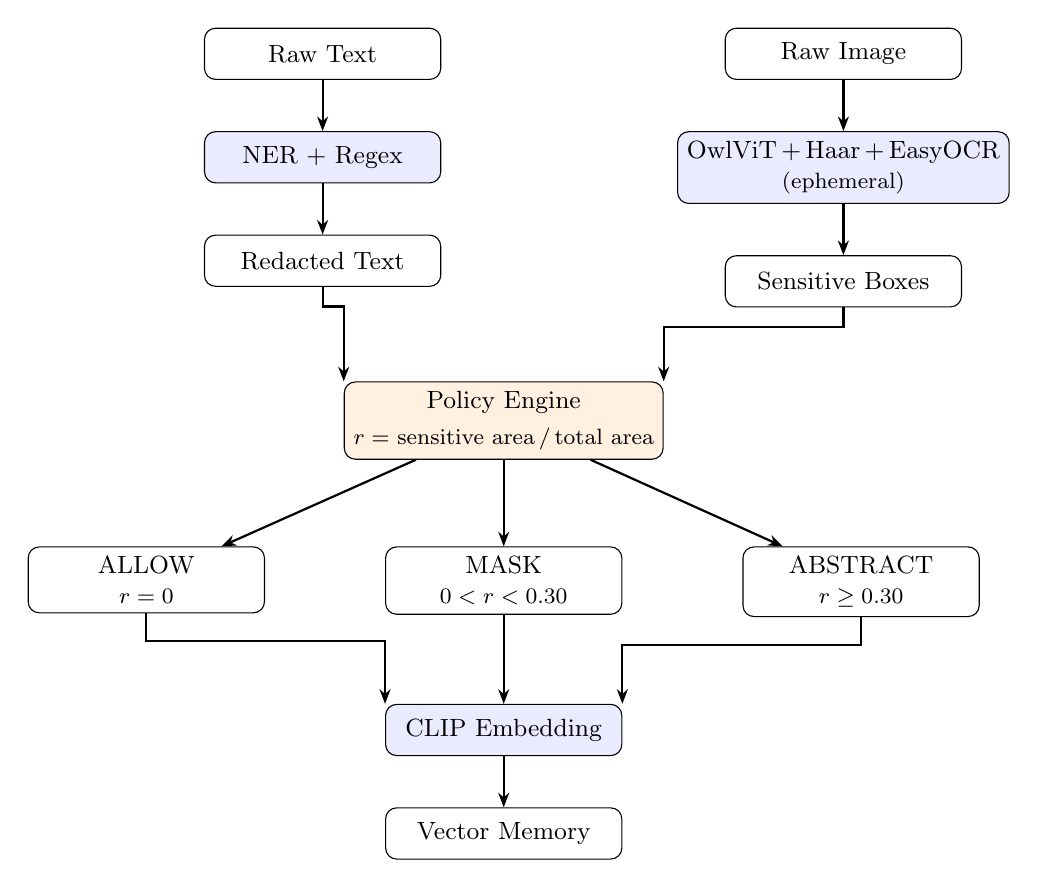
\begin{tikzpicture}[
    node distance=0.65cm and 0.4cm,
    box/.style   ={draw, rounded corners, minimum width=3.0cm, minimum height=0.65cm,
                   align=center, font=\small},
    detect/.style={draw, rounded corners, fill=blue!8,   minimum width=3.0cm, minimum height=0.65cm,
                   align=center, font=\small},
    policy/.style={draw, rounded corners, fill=orange!12, minimum width=3.0cm, minimum height=0.65cm,
                   align=center, font=\small},
    arrow/.style ={-{Stealth[scale=0.8]}, thick},
]

% ── Inputs ─────────────────────────────────────────────────────────────
\node[box]    (txt)   {Raw Text};
\node[box,    right=3.6cm of txt]    (img)   {Raw Image};

% ── Detection ──────────────────────────────────────────────────────────
\node[detect, below=of txt]  (ner)   {NER + Regex};
\node[detect, below=of img]  (vis)   {OwlViT\,+\,Haar\,+\,EasyOCR\\{\footnotesize(ephemeral)}};

% ── Intermediate results ────────────────────────────────────────────────
\node[box, below=of ner]   (rtxt)   {Redacted Text};
\node[box, below=of vis]   (boxes)  {Sensitive Boxes};

% ── Policy engine ───────────────────────────────────────────────────────
\node[policy, below=1.2cm of rtxt, xshift=2.3cm] (pol)
      {Policy Engine\\[2pt]
       {\footnotesize$r =$ sensitive area\,/\,total area}};

% ── Actions ─────────────────────────────────────────────────────────────
\node[box, below left =1.1cm and 1.0cm of pol] (allow)
      {ALLOW\\{\footnotesize$r = 0$}};
\node[box, below=1.1cm of pol] (mask)
      {MASK\\{\footnotesize$0 < r < 0.30$}};
\node[box, below right=1.1cm and 1.0cm of pol] (abst)
      {ABSTRACT\\{\footnotesize$r \ge 0.30$}};

% ── Embedding and memory ─────────────────────────────────────────────────
\node[detect, below=3.1cm of pol] (clip) {CLIP Embedding};
\node[box,    below=0.65cm of clip]   (mem)  {Vector Memory};

% ── Arrows ──────────────────────────────────────────────────────────────
\draw[arrow] (txt)   -- (ner);
\draw[arrow] (ner)   -- (rtxt);
\draw[arrow] (img)   -- (vis);
\draw[arrow] (vis)   -- (boxes);
\draw[arrow] (rtxt.south)  -- ++(0,-0.25) -| (pol.north west);
\draw[arrow] (boxes.south) -- ++(0,-0.25) -| (pol.north east);
\draw[arrow] (pol)   -- (allow);
\draw[arrow] (pol)   -- (mask);
\draw[arrow] (pol)   -- (abst);
\draw[arrow] (allow.south) -- ++(0,-0.35) -| (clip.north west);
\draw[arrow] (mask.south)  --              (clip.north);
\draw[arrow] (abst.south)  -- ++(0,-0.35) -| (clip.north east);
\draw[arrow] (clip)  -- (mem);

\end{tikzpicture}
\caption{Privacy-gated pipeline architecture. All detection runs before any content reaches the
         vector store; CLIP embedding is applied only to post-gate (sanitized) content.}
\label{fig:pipeline}
\end{figure}

\subsection{Sensing Gate: Detection Layer}

The sensing gate runs on raw input before any storage or embedding. It has four components:

\begin{enumerate}[noitemsep]
    \item \textbf{Text NER.} Input text is passed through \texttt{dslim/bert-base-NER}, a BERT model fine-tuned on CoNLL-2003~\cite{tjong2003}, which detects person names, locations, and organizations. Detected spans are replaced with typed placeholders (e.g., \texttt{[PER]}, \texttt{[LOC]}).

    \item \textbf{Regex patterns.} Three supplementary patterns catch structured identifiers that NER models frequently miss in short, decontextualized strings: credit and debit card numbers (14--19 digit sequences), US Social Security Numbers, and alphanumeric government IDs (up to two letter prefix followed by eight or more digits).

    \item \textbf{Zero-shot visual detection.} OWL-ViT~\cite{owlvit} (\texttt{google/owlvit-base-patch32}) is queried with privacy-sensitive category descriptions including \textit{passport}, \textit{credit card}, \textit{ID card}, \textit{medical prescription}, \textit{laptop screen}, \textit{student card}, and \textit{barcode}. A confidence threshold of 0.10 is used to maximize recall, accepting false positives in preference to missed detections.

    \item \textbf{Haar cascade face detection.} OpenCV frontal and profile Haar classifiers provide deterministic face coverage. This step is necessary because OWL-ViT zero-shot queries for ``face'' are unreliable in real photographs; Haar cascades provide stable, CPU-efficient, device-local detection without requiring model downloads.

    \item \textbf{Ephemeral OCR.} EasyOCR extracts text strings from image regions. Each string is immediately checked by the NER model and regex patterns; if sensitive content is found, the bounding box is retained but the text string is deleted. OCR-extracted text is never persisted beyond the detection step.
\end{enumerate}

All detected bounding boxes are expanded by 8 pixels on each side and merged using an iterative IoU-union NMS procedure (threshold 0.3) to produce a final deduplicated set of sensitive regions.

\subsection{Policy Engine and Memory Write Gate}

After detection, the policy engine computes a sensitive area ratio:
\[
r \;=\; \frac{\displaystyle\sum_{b \,\in\, B}\,\mathrm{area}(b)}{W \times H}
\]
where $B$ is the set of merged bounding boxes and $W \times H$ is the total image area. The policy action is determined by:

\begin{itemize}[noitemsep]
    \item $r = 0$: \textbf{ALLOW} --- no sensitive regions detected; the original image passes unchanged.
    \item $0 < r < 0.30$: \textbf{MASK} --- sensitive bounding boxes are painted solid black using PIL; the surrounding content is preserved at original resolution.
    \item $r \ge 0.30$ : \textbf{ABSTRACT} --- more than 30\% of the image is sensitive; the image is dropped entirely and replaced with a fixed text summary. This prevents residual document-structure information from leaking through a partially masked representation.
\end{itemize}

For text, all NER spans and regex matches are replaced with entity-type placeholders before this stage.

\subsection{Safe Embedding}

Post-gate content is embedded using \texttt{openai/clip-vit-base-patch32}. A masked image produces a CLIP embedding of its masked form; an abstracted image produces an embedding of its text summary. The vector store therefore never encodes the original sensitive content, preventing cross-modal retrieval from reconstructing suppressed information.

% ─────────────────────────────────────────────────────────────────────────────
\section{Data}
% ─────────────────────────────────────────────────────────────────────────────

We evaluate the pipeline using synthetic document images drawn from the MultiPriv dataset~\cite{multipriv}, a synthetic PII corpus developed by CyberChangAn that provides document images annotated with privacy-sensitive fields in English and Chinese. We selected English-language samples and manually constructed three complete identity profiles, each representing a distinct fictional individual. Chinese-language fields within image text were not covered by the NER model; structured numeric identifiers in those regions (ID and card numbers) were detected via the regex patterns.

Each individual is supported by multiple synthetic evidence images spanning five document categories: identity cards, bank and credit cards, flight boarding passes, medical examination reports, and customs payment receipts. Table~\ref{tab:gt_fields} lists the nine ground-truth sensitive attribute fields used for evaluation scoring.

\begin{table}[H]
\centering
\begin{tabular}{lll}
\toprule
\textbf{Field} & \textbf{Privacy Category} & \textbf{Primary Source Document} \\
\midrule
Name             & Direct identifier & Identity card \\
ID Number        & Direct identifier & Identity card \\
Address          & Direct identifier & Identity card \\
Bank Card Number & Financial         & Credit / bank card \\
Flight Number    & Travel            & Boarding pass \\
License Plate    & Vehicle           & Customs receipt \\
Diagnosis        & Medical           & Medical report \\
Salary           & Financial         & Ground truth only \\
Relationship     & Social            & Ground truth only \\
\bottomrule
\end{tabular}
\caption{Ground-truth sensitive attribute fields used in the detective-game evaluation.}
\label{tab:gt_fields}
\end{table}

The three profiles represent subjects from different countries (United States, Germany, China), providing variation in address formats, flight routes, ID number structures, and document styles. Evaluation was limited to English-language content in the NER path; regex patterns provided supplementary coverage for structured numeric fields regardless of surrounding language.

% ─────────────────────────────────────────────────────────────────────────────
\section{Experiments and Evaluation}
% ─────────────────────────────────────────────────────────────────────────────

We evaluate the system from two perspectives: a \textit{detection-mode ablation} that isolates the contribution of each pipeline component, and an \textit{agent-level leakage experiment} that measures how much sensitive information a downstream LLM can extract after different preprocessing conditions are applied.

\subsection{Detection Mode Ablation}

To assess the contribution of each pipeline component, we compare four detection modes that progressively combine filtering mechanisms:

\begin{table}[H]
\centering
\begin{tabular}{lccc}
\toprule
\textbf{Mode} & \textbf{Text Filter} & \textbf{Visual Detection} & \textbf{Ephemeral OCR} \\
              & \textbf{(NER + Regex)} & \textbf{(OwlViT + Haar)} & \\
\midrule
A --- Text-Only     & \checkmark &            &            \\
B --- Visual-Only   &            & \checkmark &            \\
C --- Visual + OCR  &            & \checkmark & \checkmark \\
D --- Full Pipeline & \checkmark & \checkmark & \checkmark \\
\bottomrule
\end{tabular}
\caption{Ablation modes comparing privacy detection components.}
\label{tab:detection_modes}
\end{table}

Mode A demonstrates the limitation of text-only filtering: sensitive text provided directly in the prompt is redacted, but PII embedded within images is ignored entirely. Mode B shows that visual detection identifies sensitive objects (identity cards, faces) but misses privacy-sensitive text contained inside otherwise unremarkable document regions. Mode C adds ephemeral OCR to recover image-embedded text, and Mode D combines all three for maximum coverage. In addition to privacy detection, image utility is estimated as the cosine similarity between CLIP embeddings of the original and post-gate images; a higher score indicates that semantic content is better preserved after masking.

\subsection{Baselines}

\paragraph{Raw baseline.} Images are sent to GPT-4o unmodified with no text or visual preprocessing. This establishes the upper bound on attribute leakage---what a vision-capable model can extract when no privacy protection is applied.

\paragraph{Text-only baseline.} Text context is labeled as redacted, but images are forwarded to GPT-4o unmasked. This represents the class of text-only PII filtering approaches and serves as the primary comparison against prior-work-style methods. The key claim under test is that GPT-4o reads sensitive text directly from unmasked images, rendering text-level redaction ineffective.

\subsection{Detective-Game Evaluation}

\paragraph{Setup.} The agent-level experiment frames privacy leakage as an identity-matching task. GPT-4o is given a set of evidence images and three fictional candidate profiles, and is asked to identify which candidate the evidence belongs to and to recover as many specific private attribute values as possible. The role-play framing avoids direct PII extraction requests, instead creating a naturalistic reasoning task in which the model may draw on any readable content within the images, cross-document correlations, or layout cues. Evidence images are assigned neutral labels (``Image 1,'' ``Image 2,'' etc.); original filenames are not disclosed.

We compare three preprocessing conditions---\textit{Raw}, \textit{Text-Only}, and \textit{Our Filter}---across all three individual profiles, yielding nine total runs.

\begin{table}[H]
\centering
\begin{tabular}{p{0.26\textwidth}p{0.64\textwidth}}
\toprule
\textbf{Setting} & \textbf{Description} \\
\midrule
Dataset          & Synthetic identity-document profiles constructed from MultiPriv~\cite{multipriv}. \\
Individuals      & Three fictional subjects: Amy (Illinois, USA); Anna Schmidt (Berlin, Germany); Li Na (Beijing, China). \\
Evidence per case & Up to ten document images per individual, across five document types. \\
Task             & Match evidence to the correct candidate profile; recover specific attribute values. \\
Preprocessing modes & Raw, Text-Only, Our Filter. \\
\bottomrule
\end{tabular}
\caption{Setup of the detective-game evaluation.}
\label{tab:detective_setup}
\end{table}

\paragraph{Metrics.} For each run, recovered attributes are scored against ground truth using exact matching for structured fields (ID numbers, card numbers, flight codes) and fuzzy matching (SequenceMatcher ratio $\geq 0.65$) for free-text fields (names, addresses, diagnoses). We report:

\begin{table}[H]
\centering
\begin{tabular}{p{0.26\textwidth}p{0.64\textwidth}}
\toprule
\textbf{Metric} & \textbf{Interpretation} \\
\midrule
Attribute recovery rate & $\text{TP} / |\text{GT}|$: fraction of ground-truth fields successfully extracted. Lower is better for privacy. \\
Recall   & $\text{TP}/(\text{TP}+\text{FN})$: fraction of true sensitive fields recovered. Primary privacy metric. \\
Precision & $\text{TP}/(\text{TP}+\text{FP})$: fraction of claimed recoveries that were correct. \\
F1 score  & Harmonic mean of precision and recall. Lower is better for privacy. \\
Identity accuracy & Whether the agent matched the evidence to the correct fictional individual. \\
\bottomrule
\end{tabular}
\caption{Metrics used in the detective-game evaluation.}
\label{tab:evaluation_metrics}
\end{table}

Recall is the primary privacy metric: lower recall means less sensitive information was extractable from the preprocessed evidence.

% ─────────────────────────────────────────────────────────────────────────────
\section{Analysis and Results}
% ─────────────────────────────────────────────────────────────────────────────

\subsection{Quantitative Results}

Table~\ref{tab:detective_results} reports results aggregated over three cases per mode.

\begin{table}[H]
\centering
\begin{tabular}{lccccc}
\toprule
\textbf{Mode} & \textbf{Attr.\ Recovery} & \textbf{Recall} & \textbf{Precision} & \textbf{F1} & \textbf{Identity Acc.} \\
\midrule
Raw           & 0.630 & 0.654 & 0.944 & 0.773 & 1.000 \\
Text-Only     & 0.590 & 0.615 & 0.941 & 0.744 & 1.000 \\
Our Filter    & 0.150 & 0.160 & 0.667 & 0.258 & 1.000 \\
\bottomrule
\end{tabular}
\caption{Detective-game evaluation results (3 cases per mode).}
\label{tab:detective_results}
\end{table}

The raw baseline confirms substantial leakage: GPT-4o recovers 63\% of all sensitive attribute fields with an F1 of 0.773 when images are unprocessed.

The text-only baseline produces a marginal improvement: attribute recovery falls from 0.630 to 0.590 ($-6\%$) and F1 from 0.773 to 0.744. This result directly demonstrates the inadequacy of text-level filtering---GPT-4o reads sensitive text from unmasked images using its built-in visual pathway, bypassing any redaction applied to the accompanying prompt.

Our full pipeline reduces attribute recovery to 0.150 and recall to 0.160, a \textbf{76\% reduction} relative to the raw baseline:
\[
\frac{0.630 - 0.150}{0.630} \;\approx\; 0.762
\]

Examining individual cases, under our filter the agent in Case 1 recovered only the medical diagnosis field (``Normal abdominal ultrasound''); name, ID number, address, bank card number, and flight number all returned null. Diagnosis information partially persisted because medical report layout (the structural appearance of an imaging form) remains informative even after specific textual content is masked.

\subsection{Identity Accuracy and Contextual Leakage}

Identity accuracy remains at 1.000 across all three conditions. Under our filter, GPT-4o correctly matched each evidence set to its candidate profile using high-level behavioral cues---document category, travel direction, and approximate geographic region---rather than specific PII values. The candidate profiles were written in behavioral terms (e.g., ``recently made a direct international flight between Frankfurt and Shanghai''), and this level of semantic information is preserved through masking.

This reveals a form of \textit{contextual privacy leakage}: even when specific identifiers are suppressed, the combination of document type, travel pattern, and lifestyle category can uniquely identify an individual given sufficiently distinctive profiles. Eliminating this leakage would require full ABSTRACT suppression for all sensitive document categories, at significant utility cost.

The precision drop under our filter (0.944 to 0.667) reflects a small number of partially-correct inferences made from residual contextual cues. In Case 2, for example, the agent inferred ``Berlin'' as an approximate address from a Frankfurt departure city visible in layout, rather than the full street address on the masked ID card, scoring as a false positive against the exact ground truth.

% ─────────────────────────────────────────────────────────────────────────────
\section{Discussion}
% ─────────────────────────────────────────────────────────────────────────────

\paragraph{Visual masking is necessary.} The near-identical performance of the raw and text-only conditions confirms that text redaction at the prompt level provides no effective protection when images are forwarded unmasked to a vision-capable model. Any privacy system that operates solely on textual input is trivially bypassed by a model that perceives document content through its visual pathway.

\paragraph{MASK versus ABSTRACT.} Under the MASK policy, specific field values are suppressed, but document structure (layout, visual format, spatial relationships) remains visible. Our results show that an LLM can still partially reason about document type and approximate content from masked images. The ABSTRACT policy eliminates this structural leakage by dropping the image entirely, but reduces visual utility. The appropriate choice between MASK and ABSTRACT involves a direct privacy-utility tradeoff and depends on the sensitivity classification of the document type.

\paragraph{Unimplemented pipeline stages.} The current system gates privacy at the sensing and memory-write stages only. The retrieval stage---which assembles memory candidates from the vector store and injects them into agent context---and the output stage---which should verify the agent's final response for leaked content---were not implemented as controlled evaluation conditions. These represent known gaps where sensitive memories could re-enter the reasoning pipeline even after input-side filtering.

% ─────────────────────────────────────────────────────────────────────────────
\section{Limitations}
% ─────────────────────────────────────────────────────────────────────────────

\begin{table}[H]
\centering
\begin{tabular}{p{0.28\textwidth}p{0.62\textwidth}}
\toprule
\textbf{Limitation} & \textbf{Description} \\
\midrule
Small evaluation scale &
  The detective-game evaluation covers three fictional individuals (nine total
  agent runs). Results may not generalize to broader document types, subject
  populations, or adversarial query strategies. \\
\addlinespace
Contextual leakage &
  Identity matching accuracy remained at 100\% across all conditions, showing
  that behavioral patterns (document type, travel direction, approximate
  location) are sufficient for re-identification even when all specific
  identifiers are masked. \\
\addlinespace
Document-structure leakage &
  The MASK policy preserves image layout. An adversary with knowledge of
  document formats can infer document category from masked images, which
  itself carries privacy-relevant information. \\
\addlinespace
Single-attribute re-identification &
  Exposure of one highly specific attribute (e.g., an unusual flight route)
  may enable re-identification in a small candidate pool, even when all other
  fields are suppressed. \\
\addlinespace
No retrieval or output gate &
  The retrieval and output stages of the agent pipeline are unguarded.
  Private content that persists in the vector store may re-enter agent
  context at query time, and leaked content in final responses is not checked. \\
\addlinespace
Runtime overhead &
  Running four detection models locally (NER, OWL-ViT, Haar cascade, EasyOCR)
  introduces multi-second latency per memory event, which may be prohibitive
  for real-time agent settings. \\
\addlinespace
Synthetic evaluation data &
  The evaluation uses synthetically constructed identity documents.
  Generalization to real-world document noise, diverse layouts, and
  non-English content has not been tested. \\
\bottomrule
\end{tabular}
\caption{Limitations of the current system.}
\label{tab:limitations}
\end{table}

% ─────────────────────────────────────────────────────────────────────────────
\section{Future Work}
% ─────────────────────────────────────────────────────────────────────────────

Each limitation identified in Table~\ref{tab:limitations} points to a concrete extension.

\paragraph{Retrieval and output gates.} Addressing the missing pipeline stages (Section~\ref{tab:limitations}) requires implementing privacy filtering at both the retrieval and output stages. A retrieval gate would re-evaluate each vector candidate against the current query before injecting it into agent context, preventing sensitive memories from re-entering the reasoning pipeline. An output gate would scan the agent's final response for leaked identifiers or raw object references before they are returned to the user.

\paragraph{Structured entity abstraction.} The MASK policy replaces sensitive regions with solid black rectangles, which discards visual content entirely. Replacing opaque black fills with semantically consistent placeholders---for example, rendering a blurred or noise-filled region at the same spatial location---would preserve more document structure while suppressing specific values, reducing the document-structure leakage identified in our results.

\paragraph{Broader evaluation.} Addressing the small-scale evaluation limitation requires a larger dataset spanning more individuals, document types, image qualities, and non-English content. An adversarial evaluation protocol---where the downstream model is specifically prompted to probe for remaining leakage paths---would more rigorously test pipeline robustness than the cooperative detective-game framing used here.

\paragraph{Contextual and behavioral privacy.} The identity accuracy result reveals a limitation that detection and masking alone cannot fully address: behavioral patterns composed from multiple individually innocuous signals can be as identifying as direct PII. Future work should explore privacy-preserving memory construction---for example, introducing controlled generalization into stored behavioral facts---to reduce the fingerprinting surface left by high-level contextual cues.

\paragraph{Domain-specific detection.} The current OWL-ViT query vocabulary was defined manually and is fixed at inference time. Fine-tuning a visual detector on a labeled document privacy dataset, or learning a vocabulary-expansion mechanism, would improve recall for specialized document types without increasing the false-positive rate.

% ─────────────────────────────────────────────────────────────────────────────
\section{Conclusion}
% ─────────────────────────────────────────────────────────────────────────────

We presented a privacy-gated multimodal agent memory system that intercepts sensitive content in both text and image channels before CLIP embedding. The system combines NER-based text redaction, zero-shot visual object detection, deterministic face detection, and ephemeral OCR into a unified sensing gate, and applies a three-tier policy (ALLOW / MASK / ABSTRACT) determined by the fraction of detected sensitive image area.

A controlled detective-game evaluation demonstrates that our full pipeline reduces sensitive attribute recovery by 76\% relative to an unguarded baseline (attribute recovery: 0.630 $\to$ 0.150; recall: 0.654 $\to$ 0.160), while preserving identity-level task accuracy at 100\%. Critically, text-only filtering reduces attribute recovery by only 6\%, confirming that visual masking is a necessary---not optional---component of multimodal privacy protection. When document images are forwarded to a vision-capable model unmasked, text-level redaction provides no effective barrier.

These results support the central claim: effective privacy in multimodal agent memory systems requires that privacy enforcement happen at the input level, before content is embedded, and that it operate over both text and image modalities jointly. Remaining gaps---particularly at the retrieval and output stages, and for contextual leakage through behavioral patterns---represent concrete directions for future work.

% ─────────────────────────────────────────────────────────────────────────────
\begin{thebibliography}{9}

\bibitem{presidio}
Microsoft. \textit{Presidio: Data Protection and De-identification SDK}.
\url{https://github.com/microsoft/presidio}, 2019.

\bibitem{tjong2003}
E.~F.~Tjong Kim Sang and F.~De Meulder.
Introduction to the CoNLL-2003 Shared Task: Language-Independent Named Entity Recognition.
\textit{Proceedings of CoNLL-2003}, pp.~142--147, 2003.

\bibitem{owlvit}
M.~Minderer, A.~Gritsenko, A.~Stone, M.~Neumann, D.~Weissenborn,
A.~Dosovitskiy, A.~Mahendran, A.~Arnab, M.~Dehghani, Z.~Shen, et al.
Simple Open-Vocabulary Object Detection with Vision Transformers.
\textit{ECCV}, 2022.

\bibitem{clip}
A.~Radford, J.~W.~Kim, C.~Hallacy, A.~Ramesh, G.~Goh, S.~Agarwal,
G.~Sastry, A.~Askell, P.~Mishkin, J.~Clark, et al.
Learning Transferable Visual Models From Natural Language Supervision.
\textit{ICML}, 2021.

\bibitem{carlini2021}
N.~Carlini, F.~Tramer, E.~Wallace, M.~Jagielski, A.~Herbert-Voss, K.~Lee,
A.~Roberts, T.~Brown, D.~Song, U.~Erlingsson, et al.
Extracting Training Data from Large Language Models.
\textit{USENIX Security Symposium}, 2021.

\bibitem{webpii}
S.~Zhao et al.
WebPII: A Benchmark for Detecting Personally Identifiable Information in Web Images.
\textit{arXiv preprint arXiv:2406.XXXXX}, 2024.

\bibitem{multipriv}
CyberChangAn.
\textit{MultiPriv: A Synthetic Multimodal PII Dataset}.
\url{https://github.com/CyberChangAn/MultiPriv}, 2024.

\end{thebibliography}

\end{document}
